\section{Kernel Trick}

\begin{frame}{Hạn chế của SVM tuyến tính}
  \begin{itemize}
    \item Cả Hard-Margin và Soft-Margin đều tìm \textbf{siêu phẳng tuyến tính}.
    \item Thực tế: nhiều tập dữ liệu có \textbf{ranh giới phi tuyến} (đường cong, vòng tròn).
    \item SVM tuyến tính thất bại hoàn toàn – dù có thêm slack $\xi_i$ cũng không giải quyết được.
  \end{itemize}
  \vspace{0.3cm}
  \centering
  \textbf{→ Cần một cách để mở rộng SVM sang các ranh giới phi tuyến.}
\end{frame}

\begin{frame}{Ví dụ: Dữ liệu hai vòng tròn đồng tâm}
  \begin{columns}
    \begin{column}{0.4\textwidth}
      \begin{itemize}
        \item Lớp trong (đỏ) và lớp ngoài (xanh)
        \item \textbf{Không} đường thẳng nào phân tách được hai lớp; Soft‑margin vẫn bất lực vì bản chất tuyến tính.
      \end{itemize}
    \end{column}
    \begin{column}{0.6\textwidth}
      \centering
      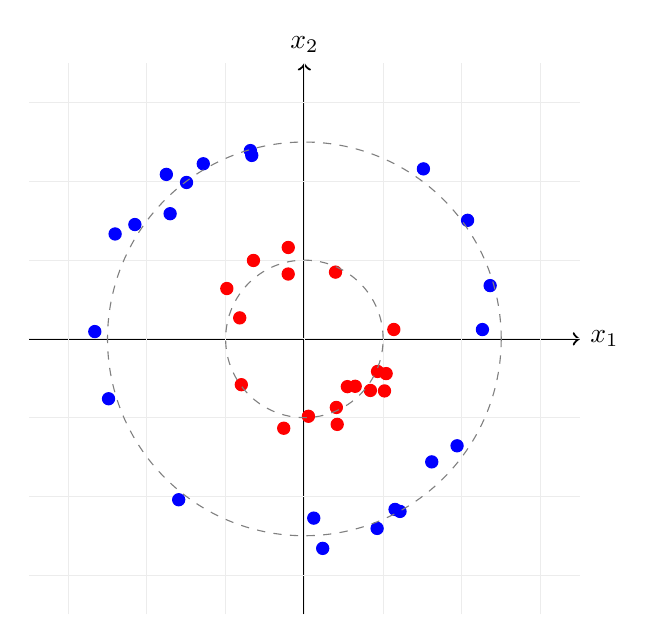
\begin{tikzpicture}[scale=1.0]
        % Trục tọa độ
        \draw[->, thick] (-3.5,0) -- (3.5,0) node[right] {$x_1$};
        \draw[->, thick] (0,-3.5) -- (0,3.5) node[above] {$x_2$};
        
        % Lưới mờ
        \draw[gray!15, thin] (-3.5,-3.5) grid (3.5,3.5);
        
        % Lớp ngoài (xanh) - bán kính ~2.5 ± nhiễu
        \foreach \i in {1,...,22} {
            \pgfmathsetmacro{\ang}{random(0,360)}
            \pgfmathsetmacro{\rad}{2.5 + 0.35*rand}
            \filldraw[blue] ({\rad*cos(\ang)}, {\rad*sin(\ang)}) circle (2.2pt);
        }
        
        % Lớp trong (đỏ) - bán kính ~1.0 ± nhiễu
        \foreach \i in {1,...,18} {
            \pgfmathsetmacro{\ang}{random(0,360)}
            \pgfmathsetmacro{\rad}{1.0 + 0.25*rand}
            \filldraw[red] ({\rad*cos(\ang)}, {\rad*sin(\ang)}) circle (2.2pt);
        }
        
        % Đường tròn tham khảo mờ
        \draw[gray, dashed, thin] (0,0) circle (1.0);
        \draw[gray, dashed, thin] (0,0) circle (2.5);
      \end{tikzpicture}
    \end{column}
  \end{columns}
\end{frame}

% ======================================
% Giới thiệu về phép phi tuyến
% ======================================

\begin{frame}{Ý tưởng: Ánh xạ đặc trưng $\phi(\mathbf{x})$}
  \begin{itemize}
    \item Ánh xạ dữ liệu từ không gian gốc $\mathbb{R}^d$ lên không gian $\mathbb{R}^D$ ($D > d$, thường $D \gg d$).
    \item Trong không gian mới, dữ liệu có thể trở nên \textbf{tuyến tính khả tách}.
  \end{itemize}
  \begin{exampleblock}{Ví dụ đơn giản}
    Với dữ liệu 2D: $X = (x_1, x_2) \in \mathbb{R}^2$, hai lớp đan xen. \\
    Ánh xạ $X' = \phi(X) = (x_1, x_2, x_1^2 + x_2^2)$ lên 3D $\rightarrow$ dùng siêu phẳng phân tách dễ dàng.
  \end{exampleblock}
  \begin{itemize}
    \item SVM trong không gian đặc trưng: thay $\mathbf{x}$ bằng $\phi(\mathbf{x})$.
  \end{itemize}
\end{frame}

\begin{frame}{Ví dụ: Ánh xạ hai vòng tròn đồng tâm}
  \begin{figure}
    \centering
    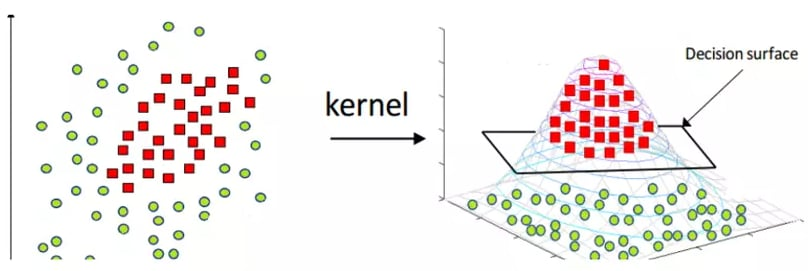
\includegraphics[width=0.7\textwidth, keepaspectratio]{img/chapter_03/kernel_trick_svm.jpg}
    \caption{Dữ liệu gốc 2D (trái) và sau khi ánh xạ lên 3D (phải)}
  \end{figure}

  
  \vspace{-0.3cm}
  \begin{columns}[T]
    \begin{column}{0.5\textwidth}
      \textbf{Không gian gốc 2D:}
      \begin{itemize}
        \item Hai lớp tạo thành vòng tròn đồng tâm.
        \item Không đường thẳng nào phân tách được.
        \item Cần ánh xạ lên không gian cao hơn.
      \end{itemize}
    \end{column}
    \begin{column}{0.5\textwidth}
      \textbf{Sau khi thêm đặc trưng $z = x_1^2 + x_2^2$:}
      \begin{itemize}
        \item Dữ liệu trải ra theo trục $z$ (bán kính).
        \item Lớp trong có $z \approx 1$, lớp ngoài $z \approx 4$.
        \item Có thể dùng một siêu phẳng (ở đây là mặt phẳng) phân tách dễ dàng.
      \end{itemize}
    \end{column}
  \end{columns}
  

\end{frame}



% ============================================
% Kernel Trick
% =============================================
\begin{frame}{Tổng quát hóa ánh xạ đặc trưng $\phi(\mathbf{x})$}
  \begin{alertblock}{Tại sao cần nhiều đặc trưng phi tuyến?}
    Trong thực tế, ta không biết trước đặc trưng nào giúp tuyến tính hóa dữ liệu. Do đó, ta thường bổ sung một tập lớn các đặc trưng:
    \[
    \phi(\mathbf{x}) = (1,\; x_1,\; x_2,\; x_1^2,\; x_2^2,\; x_1 x_2,\; \dots)
    \]
  \end{alertblock}
  
  \begin{itemize}
    \item Với $\phi(\mathbf{x})$, ta hy vọng tìm được siêu phẳng trong không gian mới phân tách tốt dữ liệu.
    \item \textbf{Nhưng:} số chiều $D$ của $\phi(\mathbf{x})$ có thể rất lớn (thậm chí vô hạn).
  \end{itemize}
\end{frame}

\begin{frame}{Thách thức của SVMs trong không gian đặc trưng}
  \begin{block}{Bài toán gốc với $\phi(\mathbf{x})$}
    \[
    \min_{\mathbf{w}, b} \frac{1}{2}\|\mathbf{w}\|^2 \quad \text{s.t.} \quad y_i(\mathbf{w}^T \phi(\mathbf{x}_i) + b) \ge 1
    \]
  \end{block}
  
  \begin{itemize}
    \item $\mathbf{w}$ có số chiều bằng với số chiều của $\phi(\mathbf{x})$, tức là $D$.
    \item Nếu $D$ rất lớn, việc lưu trữ và tính toán với $\mathbf{w}$ trở nên \textbf{bất khả thi}.
    \item Tính $\phi(\mathbf{x}_i)$ cho mọi điểm cũng cực kỳ tốn kém.
  \end{itemize}
  
  \begin{exampleblock}{Cần một cách tiếp cận khác}
    Làm sao để giải SVM mà không cần làm việc trực tiếp với vector $\mathbf{w}$ khổng lồ?
  \end{exampleblock}
\end{frame}


\begin{frame}{Bài toán đối ngẫu}
  \begin{block}{Bài toán đối ngẫu (Dual Form)}
    Khi chuyển sang bài toán đối ngẫu, vector $\mathbf{w}$ bị triệt tiêu. Hàm mục tiêu mới \textbf{chỉ phụ thuộc vào tích vô hướng} giữa các điểm trong không gian đặc trưng:
    \[
    \phi(\mathbf{x}_i)^T \phi(\mathbf{x}_j)
    \]
  \end{block}
  
  \begin{itemize}
    \item Vector trọng số được biểu diễn qua dữ liệu: $\mathbf{w} = \sum_{i} \alpha_i y_i \phi(\mathbf{x}_i)$.
    \item Hàm quyết định cũng chỉ cần tích vô hướng: $f(\mathbf{x}) = \sum_{i} \alpha_i y_i \phi(\mathbf{x}_i)^T \phi(\mathbf{x}) + b$.
  \end{itemize}
  
  \begin{alertblock}{Hệ quả then chốt}
    Nếu có cách tính $\phi(\mathbf{x}_i)^T \phi(\mathbf{x}_j)$ \textbf{trực tiếp} từ $\mathbf{x}_i, \mathbf{x}_j$ mà không cần biết $\phi$, ta sẽ giải quyết được bài toán trong không gian cao chiều một cách hiệu quả.
  \end{alertblock}
\end{frame}

% PHỤ LỤC 1 - CHỨNG MINH ĐỐI NGẪU
% \begin{frame}{Tại sao bài toán đối ngẫu chỉ cần $\phi(\mathbf{x}_i)^T \phi(\mathbf{x}_j)$?}
%   \begin{block}{Bài toán gốc trong không gian đặc trưng}
%     \[
%     \min_{\mathbf{w}, b} \frac{1}{2}\|\mathbf{w}\|^2 \quad \text{s.t.} \quad y_i(\mathbf{w}^T \phi(\mathbf{x}_i) + b) \ge 1, \forall i
%     \]
%   \end{block}

%   \begin{itemize}
%     \item Dùng phương pháp nhân tử Lagrange, ta thu được \textbf{bài toán đối ngẫu}:
%   \end{itemize}

%   \begin{exampleblock}{Hàm đối ngẫu (Dual Objective)}
%     \[
%     \max_{\bm{\alpha}} \sum_{i=1}^n \alpha_i - \frac{1}{2} \sum_{i=1}^n \sum_{j=1}^n \alpha_i \alpha_j y_i y_j \textcolor{DarkBlue}{\phi(\mathbf{x}_i)^T \phi(\mathbf{x}_j)}
%     \]
%     với $\alpha_i \ge 0$ và $\sum \alpha_i y_i = 0$.
%   \end{exampleblock}
% \end{frame}

% \begin{frame}{Tại sao bài toán đối ngẫu chỉ cần $\phi(\mathbf{x}_i)^T \phi(\mathbf{x}_j)$?}
%   \begin{exampleblock}{Hàm đối ngẫu (Dual Objective)}
%     \[
%     \max_{\bm{\alpha}} \sum_{i=1}^n \alpha_i - \frac{1}{2} \sum_{i=1}^n \sum_{j=1}^n \alpha_i \alpha_j y_i y_j \textcolor{DarkBlue}{\phi(\mathbf{x}_i)^T \phi(\mathbf{x}_j)}
%     \]
%     với $\alpha_i \ge 0$ và $\sum \alpha_i y_i = 0$.
%   \end{exampleblock}

%   \begin{itemize}
%     \item \textbf{Nhận xét:} Vector $\mathbf{w}$ đã bị triệt tiêu. Toàn bộ bài toán chỉ còn phụ thuộc vào \textbf{tích vô hướng} $\phi(\mathbf{x}_i)^T \phi(\mathbf{x}_j)$.
%     \item Hàm quyết định cũng chỉ cần tích vô hướng:
%     \[
%     f(\mathbf{x}) = \sum_{i=1}^n \alpha_i y_i \textcolor{DarkBlue}{\phi(\mathbf{x}_i)^T \phi(\mathbf{x})} + b
%     \]
%   \end{itemize}

%   \begin{alertblock}{Hệ quả quan trọng}
%     Nếu có cách tính $\phi(\mathbf{x}_i)^T \phi(\mathbf{x}_j)$ \textbf{trực tiếp} từ $\mathbf{x}_i, \mathbf{x}_j$ mà không cần biết $\phi$, ta sẽ tiết kiệm được chi phí tính toán khổng lồ.
%   \end{alertblock}
% \end{frame}


\begin{frame}{Vấn đề phát sinh với bài toán đối ngẫu}
    \begin{alertblock}{Vấn đề phát sinh}
        \begin{itemize}
        \item Khi số chiều $D$ của $\phi(\mathbf{x})$ rất lớn (thậm chí vô hạn), việc tính trực tiếp $\phi(\mathbf{x})$ (hay kể cả $\phi(\mathbf{x}_i)^T \phi(\mathbf{x}_j)$) trở nên \textbf{bất khả thi}.
        \item SVM cần tính rất nhiều tích vô hướng – nếu $D = 10^6$, mỗi phép nhân tốn $O(D)$.
        \end{itemize}
    \end{alertblock}

\end{frame}



\begin{frame}{Kernel Trick}
  \begin{block}{Ý tưởng cốt lõi}
    Thay vì tính $\phi(\mathbf{x})$ rồi lấy tích vô hướng, ta định nghĩa một hàm \textbf{kernel} $K(\mathbf{x}_i, \mathbf{x}_j)$ sao cho:
    \[
    K(\mathbf{x}_i, \mathbf{x}_j) = \phi(\mathbf{x}_i)^T \phi(\mathbf{x}_j)
    \]
    và tính \textbf{trực tiếp} từ $\mathbf{x}_i, \mathbf{x}_j$ trong không gian gốc.
  \end{block}

  \begin{exampleblock}{Ví dụ cụ thể với $\phi(\mathbf{x}) = (x_1^2, \sqrt{2}x_1 x_2, x_2^2)$}
    \begin{itemize}
      \item Tích vô hướng trong không gian đặc trưng: $\phi(\mathbf{x})^T \phi(\mathbf{z}) = x_1^2 z_1^2 + 2 x_1 x_2 z_1 z_2 + x_2^2 z_2^2 = (\mathbf{x}^T \mathbf{z})^2$
      \item Vậy chỉ cần dùng \textbf{kernel đa thức bậc 2}: $K(\mathbf{x}, \mathbf{z}) = (\mathbf{x}^T \mathbf{z})^2$.
    \end{itemize}
  \end{exampleblock}

  \begin{itemize}
    \item Chi phí tính toán: $O(d)$ trong không gian gốc thay vì $O(D)$ với $D \gg d$ (thậm chí $D = \infty$).
    \item Kernel phải thỏa mãn \textbf{điều kiện Mercer} (đảm bảo tồn tại không gian đặc trưng tương ứng).
  \end{itemize}
\end{frame}

\begin{frame}{Một số kernel phổ biến}
  \begin{columns}[T]
    \begin{column}{0.5\textwidth}
      \textbf{Linear Kernel}
      \[
      K(\mathbf{x}_i, \mathbf{x}_j) = \mathbf{x}_i^T \mathbf{x}_j
      \]
      \begin{itemize}
        \item Tương đương SVM tuyến tính.
        \item Dùng khi dữ liệu gần tuyến tính.
      \end{itemize}
      \vspace{0.3cm}
      \textbf{Polynomial Kernel}
      \[
      K(\mathbf{x}_i, \mathbf{x}_j) = (\gamma \mathbf{x}_i^T \mathbf{x}_j + r)^d
      \]
      \begin{itemize}
        \item $d$: bậc đa thức.
        \item Phù hợp với ranh giới dạng đa thức.
      \end{itemize}
    \end{column}
    \begin{column}{0.5\textwidth}
      \textbf{RBF (Gaussian) Kernel}
      \[
      K(\mathbf{x}_i, \mathbf{x}_j) = \exp\left(-\gamma \|\mathbf{x}_i - \mathbf{x}_j\|^2\right)
      \]
      \begin{itemize}
        \item Kernel được dùng \textbf{nhiều nhất}.
        \item Tương ứng không gian đặc trưng vô hạn chiều.
        \item $\gamma > 0$: tham số điều chỉnh độ phức tạp.
      \end{itemize}
    \end{column}
  \end{columns}
\end{frame}

\begin{frame}{Ảnh hưởng của $\gamma$ trong RBF Kernel}
  \begin{figure}
    \centering
    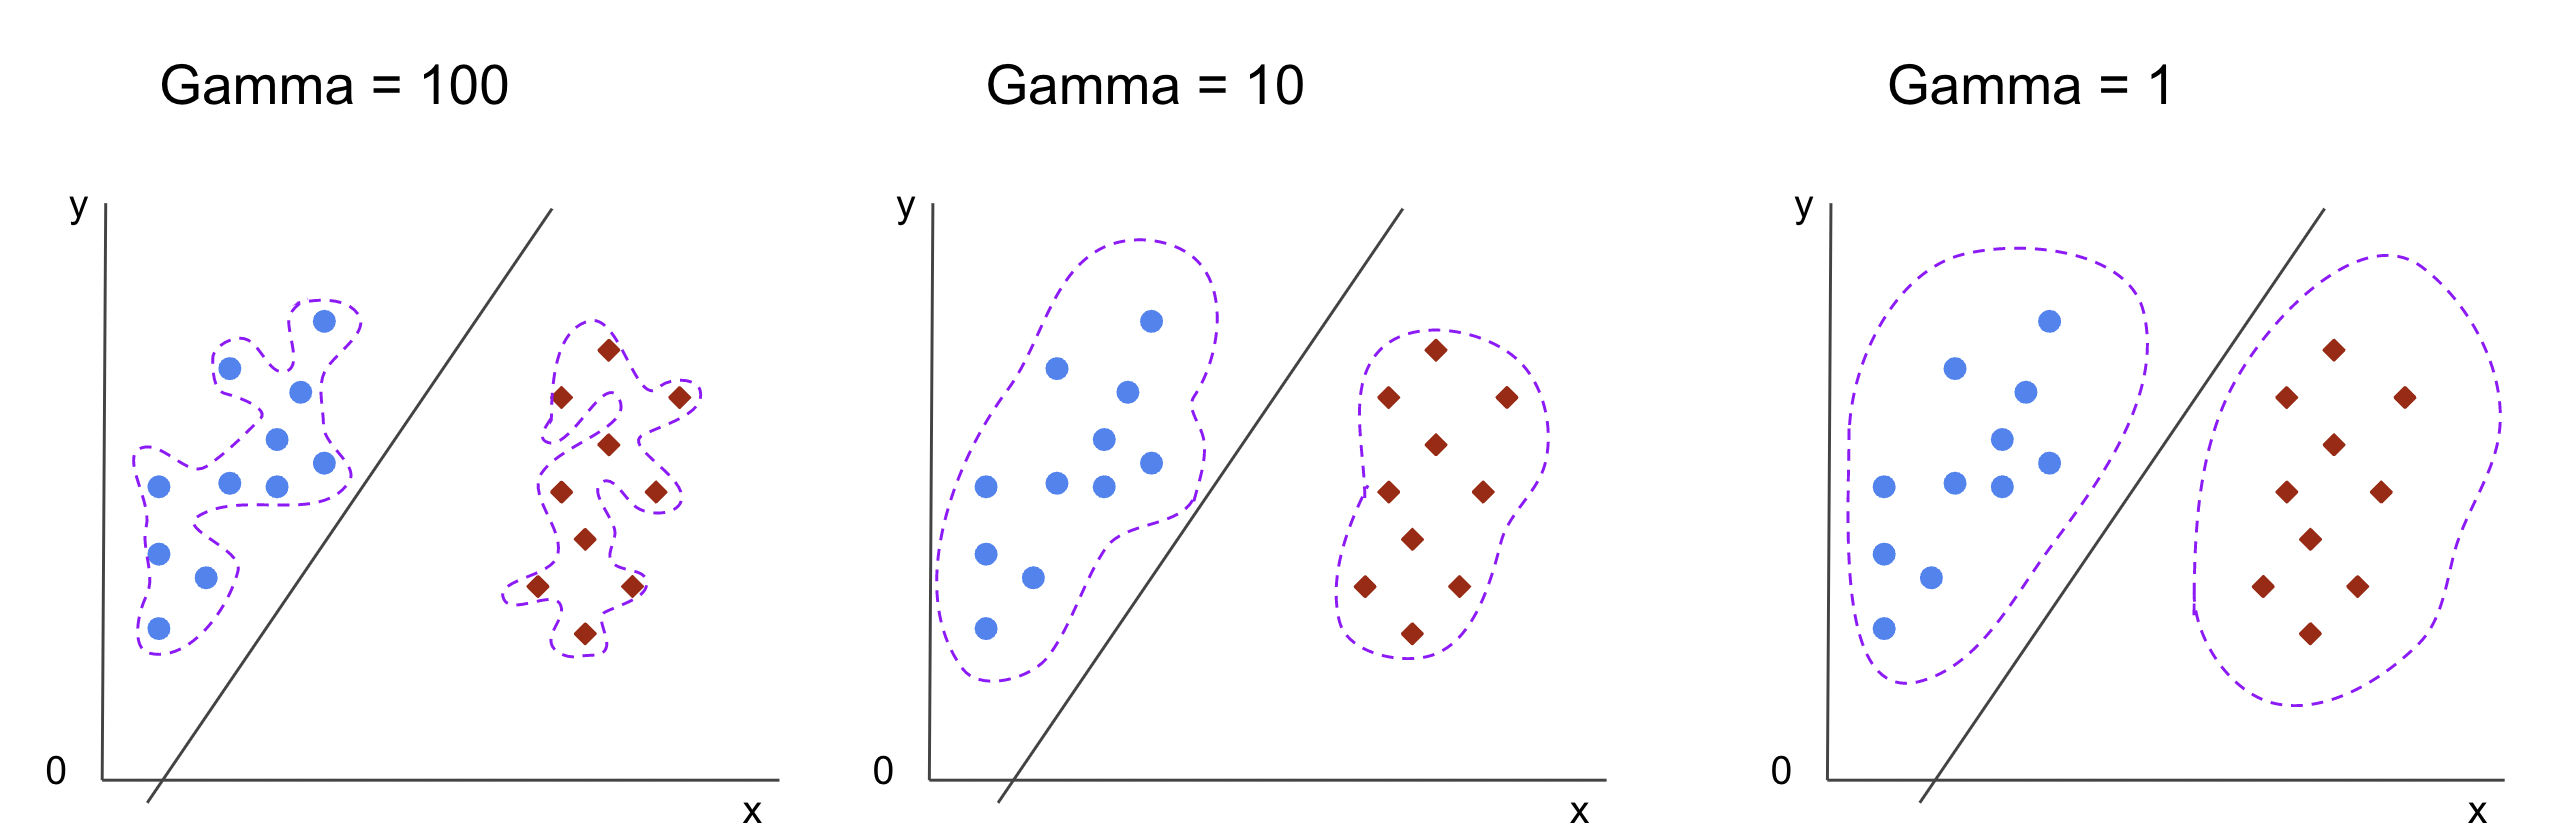
\includegraphics[width=0.8\textwidth, keepaspectratio]{img/chapter_03/gamma.png}
    \caption{Minh họa ranh giới phân loại với $\gamma$ lớn (trái) và $\gamma$ nhỏ (phải)}
  \end{figure}
  \vspace{-0.2cm}
  \begin{columns}[T]
    \begin{column}{0.5\textwidth}
      \begin{itemize}
        \item $\gamma$ \textbf{nhỏ}: mỗi điểm ảnh hưởng rộng, ranh giới mượt, tổng quát hóa tốt.
      \end{itemize}
    \end{column}
    \begin{column}{0.5\textwidth}
      \begin{itemize}
        \item $\gamma$ \textbf{lớn}: mỗi điểm ảnh hưởng hẹp, ranh giới uốn theo dữ liệu, dễ overfitting.
      \end{itemize}
    \end{column}
  \end{columns}
\end{frame}

\begin{frame}{Tối ưu siêu tham số cho SVM với kernel}
  \begin{itemize}
    \item SVM với kernel (đặc biệt là RBF) có hai siêu tham số quan trọng:
      \begin{enumerate}
        \item \textbf{$C$}: cân bằng giữa độ rộng margin và mức phạt sai số.
        \item \textbf{$\gamma$}: kiểm soát độ phức tạp của ranh giới (độ uốn).
      \end{enumerate}
    \item Chọn thủ công khó đạt hiệu quả tối ưu.
  \end{itemize}

  \begin{block}{Phương pháp phổ biến: Grid Search kết hợp Cross-Validation}
    \begin{itemize}
      \item Thử nhiều cặp $(C, \gamma)$ trên lưới giá trị (ví dụ: $C \in \{0.1, 1, 10, 100\}$, $\gamma \in \{0.001, 0.01, 0.1, 1\}$).
      \item Đánh giá bằng cross‑validation, chọn cặp cho điểm tốt nhất.
      \item Trong thư viện \texttt{scikit-learn}: \texttt{GridSearchCV(SVC(), param\_grid, cv=5)}.
    \end{itemize}
  \end{block}
\end{frame}


\begin{frame}{Tổng kết: Kernel Trick}
  \begin{block}{Vấn đề}
    \textbf{SVM tuyến tính} (cả hard và soft margin) thất bại với dữ liệu có ranh giới phi tuyến.
  \end{block}
  \begin{block}{Giải pháp}
    \begin{itemize}
      \item Ánh xạ dữ liệu lên không gian đặc trưng cao chiều $\phi(\mathbf{x})$ để dữ liệu trở nên tuyến tính khả tách.
      \item Nhờ \textbf{bài toán đối ngẫu}, mọi tính toán chỉ cần \textbf{tích vô hướng} $\phi(\mathbf{x}_i)^T \phi(\mathbf{x}_j)$.
    \end{itemize}
  \end{block}
  \begin{exampleblock}{Kernel Trick}
    Dùng \textbf{hàm kernel} $K(\mathbf{x}_i, \mathbf{x}_j)$ tính trực tiếp tích vô hướng mà không cần biết $\phi$, cho phép làm việc với không gian vô hạn chiều (RBF) với chi phí tính toán thấp.
  \end{exampleblock}
  \begin{itemize}
    \item Hai siêu tham số chính với RBF kernel: $C$ (margin vs. sai số) và $\gamma$ (độ uốn ranh giới).
    \item Thực tế: tối ưu $(C,\gamma)$ bằng \textbf{grid-search} với \textbf{cross‑validation}.
  \end{itemize}
  \vspace{0.2cm}
  \centering
\end{frame}